
%\documentclass[a4paper]{book}
%\usepackage{mcmd}
%\begin{document}

\section{mcal - Computation Between Columns\label{sect:mcal}}
\index{mcal@mcal}

Define the computation formula at the \verb|c=| parameter, and name the new data attribute at the \verb|a=| parameter. The output of \verb|mcal| is limited to 1 result without exception to simplify the program. For details of the calculation formula, please refer to the section on “Components in the expression".


\subsection*{Format}
\verb|mcal a= c=|
\hyperref[sect:option_i]{[i=]}
\hyperref[sect:option_o]{[o=]}
\hyperref[sect:option_assert_diffSize]{[-assert\_diffSize]}
\hyperref[sect:option_assert_nullkey]{[-assert\_nullkey]}
\hyperref[sect:option_assert_nullin]{[-assert\_nullin]}
\hyperref[sect:option_assert_nullout]{[-assert\_nullout]}
\hyperref[sect:option_nfn]{[-nfn]} 
\hyperref[sect:option_nfno]{[-nfno]}  
\hyperref[sect:option_x]{[-x]}
\hyperref[sect:option_q]{[-q]}
\hyperref[sect:option_option_tmppath]{[tmpPath=]}
\hyperref[sect:option_precision]{[precision=]}
\verb|[--help]|
\verb|[--helpl]|
\verb|[--version]|\\

\subsection*{Parameters}
\begin{table}[hb]
%\begin{center}
{\small
\begin{tabular}{ll}
	\verb|a=|    & Specify the new column name to store the calculated field.\\
	\verb|c=|    & Define an expression with a combination of calculation functions available. \\
\end{tabular} 
}
\end{table} 

\subsection*{Examples}
Basic usage of \verb|mcal| is illustrated in the following example. For more information on the explanation and usage of individual functions and operators, please refer to the corresponding reference. 


\begin{Verbatim}[baselinestretch=0.7,frame=single,fontsize=\small]
# Input data (dat1.csv)
customer,quantity,unitprice
A,3,10
B,1,15
C,2,20

$ mcal c='${quantity}*${unitprice}' a=amount i=dat1.csv
customer,unit price,amount
A,3,10,30
B,1,15,15
C,2,20,40

$ mcal c='${quantity}*${unitprice}<=30' a=amountbelow30 i=dat1.csv
customer,unit price,amountbelow30
A,3,10,1
B,1,15,1
C,2,20,0

$ mcal c='if(top(),${unit price},#{}+${unitprice})' a=AccumUnitprice i=dat1.csv
customer,unitprice,AccumUnitprice
A,3,10,10
B,1,15,25
C,2,20,45
\end{Verbatim}


%\subsection*{データ形式}
%mcalは用意された関数を組合せて柔軟な計算を行うことができるコマンドである。\\
%その際、入出力のデータの型には注意する必要がある。\\
%例えば2008年8月15日を"20080815"と表している日付データに対して、
%17日を加えると結果は"20080901"となるが、数値として17を加えると結果は"20080832"となるからである。\\
%mcalには、数値、文字、日付("20080815"など)、時刻("20080815235959"など)、
%論理("真"あるいは"偽")の5つの型がある。\\

\subsection*{Considerations when using shell }

When using BASH shell on UNIX operating systems, the symbol of operators often have special meaning to the shell. For example, a shell variable is represented by the \verb|$| symbol followed by a character string. On the other hand, mcmd uses the \verb|$| symbol to refers to the value of the data field. Thus, mcmd variables is enclosed in squiggly brackets preceded by the \verb|$| symbol in order not to be misinterpreted as shell variables. 

\verb|$ mcal c='${date}-10'|

\subsection*{Error message}

\verb|#ERROR# unknown function or operator|

This error message appears when there is an error in the specified operator or function. For instance, refer to the error message from the concatenation of strings function \verb|cat|. 


\begin{Verbatim}[baselinestretch=0.7,frame=single,fontsize=\small]
 $ mcal c='cat("-",1,2)'
 ERROR : unknown function or operator: cat_SNN(cat_SN) (kgcal)
\end{Verbatim}

The string before underscore character in "cat\_SNN" indicates the function name \verb|cat|, subsequently, SNN refers to the type of the argument. S refers to string type, N refers to number type, D refers to date type, and T is the time type, B refers to boolean type. The 3 characters (SNN) specifies 3 arguments. Thus, this error message means “arguments SNN of cat function” is not registered. The second and third argument is converted to string as follows. 

\begin{Verbatim}[baselinestretch=0.7,frame=single,fontsize=\small]
 $ mcal c='cat("-","1","2")'
\end{Verbatim}

The above returns an error message with 2 characters in parenthesis (SN), this refers to specification of variable or number at the first two parameters, however, only 1 variable is expressed correctly in the function.  

%\begin{Verbatim}[baselinestretch=0.7,frame=single,fontsize=\small]
% $ mcal c='cat(${商品ID},${単価},"-")' a=商品ID-単価 i=dat1.csv o=rsl1.csv
%\end{Verbatim}

\subsection*{Related Commands}
\hyperref[sect:msel]{msel} :  Use this command to select the row from the computation result.



\section{Components in the expression\label{sec:elem}}

The four key components in \verb|mcal| includes constants, item value, operator, and function. In every component, it is important for user to understand the application of data type. \verb|mcal| handles CSV text data, all values are expressed as character strings, user can define the data type to be handled in mcal. There are five string types in mcal, they are string type ($str$), numeric type ($num$), date type ($date$), time type ($time$), boolean  type ($bool$). The following sessions illustrates how each component constitutes to the expression and how to treat the data types.  


\section{Constant}
\begin{table}[!hb]
\begin{center}
\caption{Summary of constant attributes }
{\small
  \begin{tabular}{l|l|p{5cm}l|l} \hline
Data type&Format&Description&Example\\ \hline
Numerical Value($num$)   & integer, real number string& Double precision floating point numbers is used internally            & \verb|20, 0.55, 1.5*e10|\\
Character string($str$) & "Character string"         & Character string enclosed in double quotes         & \verb|"abc" "日本語"|\\
Date ($date$)  & 0dyyyymmdd       & Add "0d" before fixed length year month day                 & \verb|0d20080923| \\
Time ($time$)  & 0tyyyymmddHHMMSS & Add "0t" before fixed length year, month, date,          & \verb|0t20080923121115|\\
		& & time, minute and second & \\
              & 0tHHMMSS         & add "0t" before fixed length time, minute and second              & \verb|0t121115|\\
              &                  & (current date stored internally)              & \\
Boolean ($bool$)  & 0b1, 0b0         & Add "0b" before "1"(true) and "0"(false) & \verb|0b1, 0b0| \\

\hline
  \end{tabular}
  }
  \end{center}
\end{table}


\section{Field value}
 Table \ref{tbl:mcal_fld} shows the different data formats in the data field, the type of CSV data varies depends on how it is used and defined by the user.

\begin{table}[!hb]
\begin{center}
\caption{Format of field\label{tbl:mcal_fld}}
{\small
  \begin{tabular}{l|l|p{5cm}l|l} \hline
Data&Format&Content of CSV Data&Example\\ \hline
Numerical value($num$)   & \$\{fieldname\}  & Integer, real number (including floating Numerical string            & \verb|${amount}, ${stockprice}|\\
Character string($str$) & \$s\{fieldname\} & Character string                                           & \verb|$s{gender}, $s{gender}|\\
Date($date$)  & \$d\{fieldname\} & Fixed length year month day (yyyymmdd)                           & \verb|$d{date}, $d{orderdate}| \\
Time($time$)  & \$t\{fieldname\} & Fixed length year month day minute second (yyyymmddHHMMSS)             & \verb|$d{time}, $d{departuretime}| \\
              &               & Fixed length hour minute second (HHMMSS)                           &\\
              &               & (current date stored internally)                 &\\
Boolean($bool$)  & \$b\{fieldname\} & The value is expressed as "1" if true and "0"  if false、& \verb|$b{condition}, $b{condition}| \\
              &               & Other cases treated as NULL               & \\

\hline
  \end{tabular}
  }
  \end{center}
\end{table}

\section{Wildcard}
Wildcard can be used in field names. For example, when using the sum function to compute the total across multiple fields with numeric labels, wildcard can be use to simplify the listing of all fields as one label. For example, if there are three columns are named \verb|A1,A2,A3| in the input data, the total sum of \verb|A1,A2,A3| can be calculated as \verb|sum(${A*})|. It is also possible to specify multiple wildcard such as the expression \verb|sum(${A*},${B*})|. 


\section{Value from Previous Row }
Use the \verb|#| symbol instead of \verb|$| to refer to values from a field in the previous row. However, the function will return null when used on the first record since there is no record preceding the first record. The specification of each data type is shown in \ref{tbl:mcal_prev} below.  


\begin{table}[!hb]
\begin{center}
\caption{Specification of retrieving values from previous row\label{tbl:mcal_prev}}
{\small
  \begin{tabular}{l|lll|} \hline
Data type&Format&Example\\ \hline
Numeric($num$)   & \#\{fieldname\}  & \verb|#{amount}, #{stockprice}|\\
Character string($str$) & \#s\{fieldname\} & \verb|#s{gender}, #s{gender}|\\
Date($date$)  & \#d\{fieldname\} & \verb|#d{date}, #d{releasedate}| \\
Time($time$)  & \#t\{fieldname\} & \verb|#d{time}, #d{departuretime}| \\
Boolean($bool$)  & \#b\{fieldname\} & \verb|#b{condition}, #b{condition}| \\

\hline
  \end{tabular}
  }
  \end{center}
\end{table}

\section{Values from Next Row}
Use the expression to obtain value from the previous record without specifying the field name to obtain the value in the next record.  The specification of the data types are shown in \ref{tbl:mcal_prev_rsl}. 

It is possible to calculate total by combining \verb|if| function with \verb|top()| function. The cumulative calculation on the amount field is shown below.  


\verb|$ mcal c='if(top(),${amount},${amount}+#{})' a=cumulativeAmount|


\begin{table}[!hb]
\begin{center}
\caption{Specification to retrieve values from previous row\label{tbl:mcal_prev_rsl}}
{\small
  \begin{tabular}{l|l|l} \hline
Data Type&Format&Example\\ \hline
Numeric($num$)   & \#\{\}  & \verb|#{}|\\
Character String($str$) & \#s\{\} & \verb|#s{}|\\
Date($date$)  & \#d\{\} & \verb|#d{}| \\
Time($time$)  & \#t\{\} & \verb|#d{}| \\
Boolean($bool$)  & \#b\{\} & \verb|#b{}| \\

\hline
  \end{tabular}
  }
  \end{center}
\end{table}


\section{Arithmetic Operators}
The \verb|+| and \verb|-| arithmetic operators can be used on numeric format strings as well as date and character format strings. The data format is shown in Table \ref{tbl:mcal_ope}. 

\begin{table}[!hb]
\begin{center}
\caption{Summary of arithmetic operators \label{tbl:mcal_ope}}
{\small
  \begin{tabular}{l|l|l|l} \hline
Operator&Format&Description&Example\\
\hline
Addition(+) & $num_1+num_2$ & Addition of numeric values   & \verb|1.5+2.3 (3.8)|\\
        & $str_1+str_2$ & Join character strings    & \verb|"150"+"円" ("150円")|\\
        & $date+num$    & $num$ days after date & \verb|0d20121130+2 (0d20121202)|\\
        & $time+num$    & $num$ seconds after time & \verb|0t095959+2 (0t100001)|\\
\hline
Substraction(-) & $num_1-num_2$   & Subtraction of numeric values      & \verb|1.5-2.3 (-1.8)|\\
        & $str_1-str_2$   & Remove substring   & \verb|"aababa"-"a"| (\verb|"bb"|)\\
        &                 & (by greedy match algorithm) & \verb|"aababa"-"aba"| (\verb|"aba"|)\\
        & $date-num$      & $num$ days before date    & \verb|0d20121202-2 (0d20121130)|\\
        & $time-num$      & $num$ seconds before time    & \verb|0t100001-2 (0t095959)|\\
        & $date_1-date_2$ & Date difference             & \verb|0d20121202-0d20121130 (2)|\\
        & $time_1-time_2$ & Time difference             & \verb|0t095959-0t100001 (-2)|\\
\hline
Multiplication (*) & $num_1*num_2$ & multiply & \verb|10*2 (20)|\\
\hline
Division (/) & $num_1/num_2$ & divide & \verb|10/2 (5)|\\
\hline
Remainder (\%) & $num_1\%num_2$ & remainder & \verb|10%3 (1)|\\
\hline
Power (\^{}) & $num_1$\^{}$num_2$ & power & \verb|10^3 (1000)|\\

\hline
  \end{tabular}
\\The results of the examples are shown in parentheses (the content is shown using constant numbers).
  }
  \end{center}
\end{table}

\section{Comparison Operators }
The comparison operators can only be used on data of the same type. Table \ref{tbl:mcal_ope_comp} shows the list of operators for numeric format data. Similarly, the operators shown in the table below can be applied to character format, date format, time format data.  


\begin{table}[!hb]
\begin{center}
\caption{Summary of comparison operators \label{tbl:mcal_ope_comp}}
{\small
  \begin{tabular}{l|l|l} \hline
Details of comparison&Format&Example\\
\hline
Equal   & $num_1==num_2$ & \verb|1.5==1.5(0b1), "abc"=="abcd" (0b0)|\\
Not equal & $num_1!=num_2$ & \verb|1.5!=1.5(0b0), "abc"=="abcd" (0b1)|\\
Greater than & $num_1>num_2$  & \verb|10>5(0b1), "abc">"abcd" (0b0)|\\
Less than & $num_1<num_2$  & \verb|10<5(0b0), "abc"<"abcd" (0b1)|\\
Above       & $num_1>=num_2$ & \verb|10>=10(0b1), "a">"" (0b1) |\\
Below      & $num_1<=num_2$ & \verb|8<=9(0b1), "a"<="a" (0b1)| \\
\hline
  \end{tabular}
\\The results of the examples are shown in parentheses (the content is shown using constant numbers).  }
  \end{center}
\end{table}


\section{Logical Operator}
The usage of the three logical operators (conjunction, disjunction, exclusive or) is shown in Table \ref{tbl:mcal_bool}. In addition the results of the combination of boolean values (1:true, 0:false)  are shown in Table \ref{tbl:mcal_and},Table \ref{tbl:mcal_or} and Table \ref{tbl:mcal_xor}. 


\begin{table}[!hb]
\begin{center}
\caption{Summary of logical operators\label{tbl:mcal_bool}}
{\small
  \begin{tabular}{l|l|l} \hline
Description&Format&Example\\
\hline
Conjunction       & $bool_1 \&\& bool_2$ & \verb|"abc"=="abc" && "xyz"=="abc" (0b0)|\\
Disjunction       & $bool_1 ||   bool_2$ & \verb/"abc"=="abc" || "xyz"=="abc" (0b1)/\\
Exclusive or	& $bool_1$ \^{}\^{} $bool_2$ & \verb|"abc"=="abc" ^^ "xyz"=="abc" (0b1)|\\
\hline
  \end{tabular}
\\The results of the examples are shown in parentheses (the content is shown using constant numbers).
  }
  \end{center}
\end{table}

\begin{table}[!hb]
\begin{center}
\begin{tabular}{ccc}

\begin{minipage}{0.3\hsize}
\begin{center}
\caption{Conjunction\label{tbl:mcal_and}}
{\small
\begin{tabular}{ccc}
\hline
$bool_1$ & $bool_2$ & Result \\
\hline
1  & 1  & 1 \\
1  & 0  & 0 \\
0  & 1  & 0 \\
0  & 0  & 0 \\
null & 1  & null \\
null & 0  & 0 \\
null & null & null \\
\hline

\end{tabular}
}
\end{center}
\end{minipage}

\begin{minipage}{0.3\hsize}
\begin{center}
\caption{Disjunction\label{tbl:mcal_or}}
{\small
\begin{tabular}{ccc}
\hline
$bool_1$ & $bool_2$ & Result \\
\hline
1  & 1  & 1 \\
1  & 0  & 1 \\
0  & 1  & 1 \\
0  & 0  & 0 \\
null & 1  & 1 \\
null & 0  & null \\
null & null & null \\
\hline
\end{tabular}
}
\end{center}
\end{minipage}

\begin{minipage}{0.30\hsize}
\begin{center}
\caption{Exclusive Or\label{tbl:mcal_xor}}
{\small
\begin{tabular}{ccc}
\hline
$bool_1$ & $bool_2$ & Result \\
\hline
1  & 1  & 0 \\
1  & 0  & 1 \\
0  & 1  & 1 \\
0  & 0  & 0 \\
null & 1  & null \\
null & 0  & null \\
null & null & null \\
\hline
\end{tabular}
}
\end{center}
\end{minipage}

\end{tabular}
\end{center}
\end{table}

\section{Operator Precedence}
The operators in Table \ref{tbl:mcal_pri_ope} are listed according to precedence order.  

The order of precedence starts from the top, operators on the same line with equal precedence are evaluated from left to right. When operators of equal precedence appear in the same expression, use parentheses to change to operator precedence and the expression to evaluated first. 

\begin{table}[!hb]
\begin{center}
\caption{Precedence of operators\label{tbl:mcal_pri_ope}}
{\small
  \begin{tabular}{c|l} \hline
Order&Operator\\ \hline
1 & \verb|*,/,%,^| \\
2 & \verb|+,-|  \\
3 & \verb|>,<,>=,<=| \\ 
4 & \verb|== ,!=|  \\
5 & \verb|&&|  \\
6 & \verb/||,^^/  \\
\hline
  \end{tabular}
  }
  \end{center}
\end{table}


\section{Function}
The following highlights the 9 types of functions in relation to numeric strings (\ref{tbl_mcal_func_num}), trigonometric function (\label{tbl:mcal_sankaku}), character strings (\ref{tbl:mcal_char}), regular expression (\ref{tbl:mcal_regex}), date / time (\ref{tbl:mcal_date}), logical (\ref{tbl:mcal_logical}), row/column information (\ref{tbl:mcal_line}), Null value (\ref{tbl:mcal_null}), data type conversion (\ref{tbl:mcal_cast}). 


\begin{table}[!hb]
\begin{center}
\caption{Summary of numerical functions \label{tbl_mcal_func_num}}
{\small
  \begin{tabular}{l|l|l|l} \hline
Section&Function name&Function&Output type\\ \hline

\ref{sect:sum}& sum($num_1,num_2,\cdots$)&
Sum&
$num$\\

\ref{sect:avg}& avg($num_1,num_2,\cdots$)&
Average&
$num$\\

\ref{sect:sqsum}& sqsum($num_1,num_2,\cdots$)&
Sum of squares&
$num$\\

\ref{sect:min}& min($num_1,num_2,\cdots$)&
Minimum value&
$num$\\

\ref{sect:max}& max($num_1,num_2,\cdots$)&
Maximum value&
$num$\\

\ref{sect:product}& product($num_1,num_2,\cdots$)&
Product&
$num$\\

\ref{sect:factorial}& factorial($num$)&
Factorial&
$num$\\

\ref{sect:gcd}& gcd($num_1$,$num_2$)&
Greatest common divisor&
$num$\\

\ref{sect:lcm}& lcm($num_1$,$num_2$)&
Least common multiple&
$num$\\

\ref{sect:sqrt}& sqrt($num$)&
Square root&
$num$\\

\ref{sect:abs}& abs($num$)&
Absolute value&
$num$\\

\ref{sect:sign}& sign($num$)&
Sign&
$num$\\

\ref{sect:int}& int($num$)&
Integer part&
$num$\\

\ref{sect:fract}& fract($num$)&
Fraction part&
$num$\\

%\ref{sect:minf}& minf()&
%利用可能な最小の実数値&
%数値\\

%\ref{sect:maxf}& maxf()&
%利用可能な最大の実数値&
%数値\\

\ref{sect:round}& round($num$,nominal value)&
Rounding up&
$num$\\

\ref{sect:floor}& floor($num$,nominal value)&
Rounding down&
$num$\\

\ref{sect:ceil}& ceil($num$,nominal value)&
Ceiling&
$num$\\

\ref{sect:power}& power($num$,exponent)&
Power&
$num$\\

\ref{sect:exp}& exp($num$)&
Exponential function&
$num$\\

\ref{sect:log}& log($num$,base)&
 logarithm &
$num$\\

\ref{sect:ln}& ln($num$)&
Natural logarithm &
$num$\\

\ref{sect:log2}& log2($num$)&
Binary logarithm&
$num$\\

\ref{sect:log10}& log10($num$)&
Common logarithm&
$num$\\

\ref{sect:dist}& dist(type,$num_1,num_2,\cdots$)&
Distance&
$num$\\

\ref{sect:distgps}& distgps(latitude1,longtitude1,latitude2,longtitude2)&
GPS distance &
$num$\\


\ref{sect:heron}& heron($num_1,num_2,\cdots$)&
Heron’s formula &
$num$\\

\ref{sect:rand}& rand([random seed])&
Uniform random number &
$num$\\

\ref{sect:randi}& randi(minimum value, maximum value[, random seed])&
Uniform random number&
$num$\\

\ref{sect:nrand}& nrand(minimum value, maximum value[, random seed])&
Normal random number&
$num$\\

\ref{sect:pi}& pi()&
Pi&
$num$\\

\ref{sect:e}& e()&
Napier's constant&
$num$\\

\ref{sect:format}& format()&
Format output&
$str$\\

\hline
  \end{tabular}
  }
  \end{center}
\end{table}


\begin{table}[!hb]
\begin{center}
\caption{List of trigonometric functions \label{tbl:mcal_sankaku}}
{\small
  \begin{tabular}{l|l|l|l} \hline
Section&Function Name&Function&Output range\\ \hline

\ref{sect:acos}& acos($num$)&
Inverse cosine &
$0\sim\pi$\\

\ref{sect:asin}& asin($num$)&
Inverse sine&
$-\pi\sim\pi$\\

\ref{sect:atan}& atan($num$)&
Inverse tangent&
$-\pi\sim\pi$\\

\ref{sect:atan2}& atan2($num_1$,$num_2$)&
Angle of coordinates ($num_1,num_2$)&
$-\pi\sim\pi$\\

\ref{sect:cos}& cos($r$)&
Cosine&
$-1.0\sim 1.0$\\

\ref{sect:sin}& sin($r$)&
Sine&
$-1.0\sim 1.0$\\

\ref{sect:tan}& tan($r$)&
Tangent&
$-\infty\sim\infty$\\

\ref{sect:degree}& degree($r$)&
Degree&
$-\pi\sim\pi$\\

\ref{sect:radian}& radian(angle)&
Enter angle as input, return radian as output &
$-\pi\sim\pi$\\

\ref{sect:cosh}& cosh($r$)&
Hyperbolic cosine&
$0\sim\infty$\\

\ref{sect:sinh}& sinh($r$)&
Hyperbolic sine&
$-\infty\sim\infty$\\

\ref{sect:tanh}& tanh($r$)&
Hyperbolic tangent&
$-1.0\sim 1.0$\\

\hline
  \end{tabular}
	\\Radian is represented by the variable $r$.
  }
  \end{center}
\end{table}


\begin{table}[!hb]
\begin{center}
\caption{Character string related functions\label{tbl:mcal_char}}
{\small
  \begin{tabular}{l|l|l|l} \hline
Section&Function name&Function&Output format\\ \hline

\ref{sect:cat}& cat($token, str_1, str_2, \cdots$)&
Merge character string&
$str$\\

\ref{sect:length}& length($str$)&
Length of character string&
$num$\\

%\ref{sect:lengthw}& lengthw($str$)&
%文字列長(ワイド文字)&
%$num$\\

\ref{sect:fixlen}& fixlen($str$,length,position,padding character)&
Fixed length conversion&
$str$\\

%\ref{sect:fixlenw}& fixlenw($str$, 長さ, 位置, padding文字)&
%固定長変換(ワイド文字)&
%$str$\\

\ref{sect:right}& right($str$,length)&
Extract substring from the end&
$str$\\
%\ref{sect:rightw}& rightw($str$,長さ)&
%文字列末尾切り出し(ワイド文字)&
%$str$\\
\ref{sect:left}& left($str$,length)&
Extract substring from the beginning&
$str$\\
%\ref{sect:leftw}& leftw($str$,長さ)&
%文字列先頭切り出し(ワイド文字)&
%$str$\\
\ref{sect:mid}& mid($str$,starting position,length)&
Extract substring  &
$str$\\
%\ref{sect:midw}& midw($str$, 開始位置, 長さ)&
%部分文字列切り出し(ワイド文字) &
%$str$\\
\ref{sect:toupper}& toupper($str$)&
Convert characters from lowercase to uppercase &
$str$\\
\ref{sect:tolower}& tolower($str$)&
Converts characters from uppercase to lowercase &
$str$\\
\ref{sect:capitalize}& capitalize($str$)&
Capitalize the first character &
$str$\\
\ref{sect:match}& match(search string,$str_1,str_2,\cdots$)&
Search for matched strings&
$bool$\\

%\ref{sect:match}& matcha(検索文字列,$str_1,str_2,\cdots$)&
%AND検索&
%$bool$\\
%\ref{sect:match}& matchs(検索文字列,$str_1,str_2,\cdots$)&
%OR部分検索&
%$bool$\\
%\ref{sect:match}& matchas(検索文字列,$str_1,str_2,\cdots$)&
%AND部分検索&
%$bool$\\

\ref{sect:hasspace}& hasspace($str$)&
Search for white-space characters&
$bool$\\

\hline
  \end{tabular}
  }
  \end{center}
\end{table}

\begin{table}[!hb]
\begin{center}
\caption{Regular expression related functions \label{tbl:mcal_regex}}
{\small
  \begin{tabular}{l|l|l|l} \hline
Section&Function name&Function&Output format\\ \hline

%\ref{sect:regexs}& regexs(文,正規表現)&
%正規表現にマッチする部分文字列が存在すれば真&文字列,文字列&論理\\
\ref{sect:regexm}& regexm($str$,regular expression)&
Match whole string&
$bool$\\

\ref{sect:regexs}& regexs($str$,regular expression)&
Match&
$bool$\\


\ref{sect:regexrep}& regexrep($str$,regular expression,replacement string)&
Replace matching character string &$str$\\

\ref{sect:regexlen}& regexlen($str$,regular expression)&
Match number of characters&
$num$\\

\ref{sect:regexpos}& regexpos($str$,regular expression)&
Start position of character&
$num$\\

\ref{sect:regexstr}& regexstr($str$,regular expression)&
Match character string&
$str$\\

\ref{sect:regexpfx}& regexpfx($str$,regular expression)&
Match prefix of character string&
$str$\\

\ref{sect:regexsfx}& regexsfx($str$,regular expression)&
Match suffix of character string &
$str$\\
 
\hline
  \end{tabular}
  }
  \end{center}
\end{table}


\begin{table}[!hb]
\begin{center}
\caption{Date and Time Related Functions\label{tbl:mcal_date}}
{\small
  \begin{tabular}{l|l|l|l} \hline
Section&Function Name&Function&Output\\ \hline

\ref{sect:today}& today()&
Today’s date&$date$\\

\ref{sect:now}& now()&
Current time&$time$\\

\ref{sect:tseconds}& tseconds($time$)&
Seconds elapsed &$num$\\

\ref{sect:leapyear}& leapyear($dt$)&
Decide leap year&$bool$\\

\ref{sect:year}& year($dt$)&
Gregorian calendar &$num$\\

\ref{sect:month}& month($dt$)&
Month&$num$\\

\ref{sect:day}& day($dt$)&
Day&$num$\\

\ref{sect:week}& week($dt$)&
Week number&$num$\\

\ref{sect:dow}& dow($dt$)&
Day of week&$num$\\

\ref{sect:time}& time($time$)&
Hour minute second&$str$\\

\ref{sect:date}& date($time$)&
Year month day&$str$\\

\ref{sect:hour}& hour($time$)&
Hour&$num$\\

\ref{sect:minute}& minute($time$)&
Minute&$num$\\

\ref{sect:second}& second($time$)&
Second&$num$\\

\ref{sect:age}& age($dt_1,dt_2$)&
Age&$num$\\

\ref{sect:diff}& diff($dt_1,dt_2$)&
Period&$num$\\

\ref{sect:uxt}& uxt($dt$)&
Convert to UNIX time&$num$(UNIX time)\\

%\ref{sect:uxt}& t2uxt($time$)&
%$time\rightarrow$UNIX時変換&$num$(UNIX時刻)\\

%\ref{sect:uxt}& uxt2d($num$)&
%UNIX時$\rightarrow date$変換&$date$\\

%\ref{sect:uxt}& uxt2t($num$)&
%UNIX時$\rightarrow time$変換&$time$\\

\ref{sect:julian}& julian($dt$)&
Convert to Julian day&$num$(Julian day)\\

%\ref{sect:julian}& t2julian($time$)&
%$time\rightarrow$ユリウス通日変換&$num$(ユリウス通日)\\

%\ref{sect:julian}& julian2d($num$)&
%ユリウス通日$\rightarrow date$変換&$date$\\

%\ref{sect:julian}& julian2t($num$)&
%ユリウス通日$\rightarrow time$変換&$time$\\

\hline
  \end{tabular}
	\\$dt$ represents either $date$ or $time$.
  }
  \end{center}
\end{table}

\begin{table}[!hb]
\begin{center}
\caption{Logical Functions\label{tbl:mcal_logical}}
{\small
  \begin{tabular}{l|l|l|l} \hline
Section&Function Name&Function&Output\\ \hline

\ref{sect:and}& and($bool_1,bool_2,\cdots)$& Conjunction&$bool$\\
\ref{sect:or}& or($bool_1,bool_2,\cdots)$  & Disjunction &$bool$\\
\ref{sect:not}& not($bool)$                & NOT   &$bool$\\
\hline
\ref{sect:if}& if($bool,num_1,num_2$)      &Check logical condition& $num$\\
\ref{sect:if}& if($bool,str_1,str_2$)      &        & $str$\\
\ref{sect:if}& if($bool,date_1,date_2)$    &        & $date$\\
\ref{sect:if}& if($bool,time_1,time_2)$    &        & $time$\\

\hline
  \end{tabular}
  }
  \end{center}
\end{table}

\begin{table}[!hb]
\begin{center}
\caption{Row/column related functions \label{tbl:mcal_line}}

{\small
  \begin{tabular}{l|l|l|l} \hline
Section&Function Name&Function&Output Format\\ \hline

\ref{sect:line}   & line()   & Return the processing line number &$num$\\
\ref{sect:top}    & top()    & Top row &$bool$\\
\ref{sect:bottom} & bottom() &Last row&$bool$\\
\ref{sect:fldsize}& fldsize()&Number of fields&$num$\\
\ref{sect:argsize}& argsize($str_1,str_2,\cdots$)&Number of arguments &$num$\\

\hline
  \end{tabular}
  }
  \end{center}
\end{table}

\begin{table}[!hb]
\begin{center}
\caption{NULL value related functions\label{tbl:mcal_null}}
{\small
  \begin{tabular}{l|l|l|l} \hline
Section&Function Name&Function&Output Format\\ \hline

\ref{sect:null}& nulln()&NULL value& $num$ \\
\ref{sect:null}& nulls()&      & $str$ \\
\ref{sect:null}& nulld()&      & $date$ \\
\ref{sect:null}& nullt()&      & $time$ \\
\ref{sect:null}& nullb()&      & $bool$ \\
\hline
\ref{sect:isnull}& isnull($num$)&NULL value check& $bool$\\
\ref{sect:isnull}& isnull($str$)&          & $bool$\\
\ref{sect:isnull}& isnull($date$)&         & $bool$\\
\ref{sect:isnull}& isnull($time$)&         & $bool$\\
\ref{sect:isnull}& isnull($bool$)&         & $bool$\\
\hline
\ref{sect:countnull}& countnull($num_1,num_2,\cdots$)& Number of NULL values & $num$\\
\ref{sect:countnull}& countnull($str_1,str_2,\cdots$)& & $num$\\
\ref{sect:countnull}& countnull($date_1,date_2,\cdots$)& & $num$\\
\ref{sect:countnull}& countnull($time_1,time_2,\cdots$)& & $num$\\
\ref{sect:countnull}& countnull($bool_1,bool_2,\cdots$)& & $num$\\

\hline
  \end{tabular}
  }
  \end{center}
\end{table}


\begin{table}[!hb]
\begin{center}
\caption{Type conversion related functions \label{tbl:mcal_cast}}
{\small
\begin{tabular}{l|l|l|l|l|l} \hline
\ref{sect:cast} & $num$       & $str$       & $date$     & $time$     & $bool$     \\
\hline
\hline
$num$  &             & n2s($num$)  &            &            & n2b($num$) \\
\hline
$str$  & s2n($str$)  &             & s2d($str$) & s2t($str$) & s2b($str$) \\
\hline
$date$ &             & d2s($date$) &            & d2t($date$)& \\
\hline
$time$ &             & t2s($time$) & t2d($time$)&            & \\
\hline
$bool$ & b2n($bool$) & b2s($bool$) &            &            & \\
\hline
  \end{tabular}
 
Each cell corresponds to the conversion function from the labels in the top row  to labels in the left column. 
\\Empty cells means that conversion function is not available. 

  }
  \end{center}
\end{table}

\section{Date and Time Format\label{sect:datetime}}
There are two data types in \verb|mcal|, namely date and time format. One is the date type and the other are date type. Time formatted data is represented with date formatted data as a set. The command uses date\_time library of boost C + + library based on the Gregorian calendar, date type uses class boost::gregorian::date, and time type uses class boost::posix\_time::ptime. For more details, refer to documentation in \href{http://www.boost.org/}{boost.org}. 

Date class is managed as a 32-bit integer internally, and supports dates ranging from January 1,1400 to December 31, 9999. Operations on date is based on the Gregorian calendar. NULL value will be returned on invalid date (for example, 2013/2/29 or 1399/12/31).

On the other hand, class ptime is managed as 64 bit. It is a time system with nano-second/micro-second resolution. The mcal command do not have an interface for time point manipulation. Class ptime is dependent on gregorian::date for the interface to the date portion of a time point, thereby enable time calculations across different dates. NULL value is returned on invalid time (e.g.18:62:11).  

MCMD deals with CSV text, date/time must be assigned as character string in the data. The command then converts character string to date and time type for processing various operations.The final result converted back to character string in the output. The string format is expressed as 8-digit fixed-length string for date (e.g. "20130911"), 14-digit fixed-length string  for time (e.g. "20130911110528") or the standard 6-digit fixed-length string (for example, "110528").

Figure \ref{fig:mcal_datetime} below shows the relationship of date type, time type and various functions. 


\begin{figure}[t!]
\begin{center}
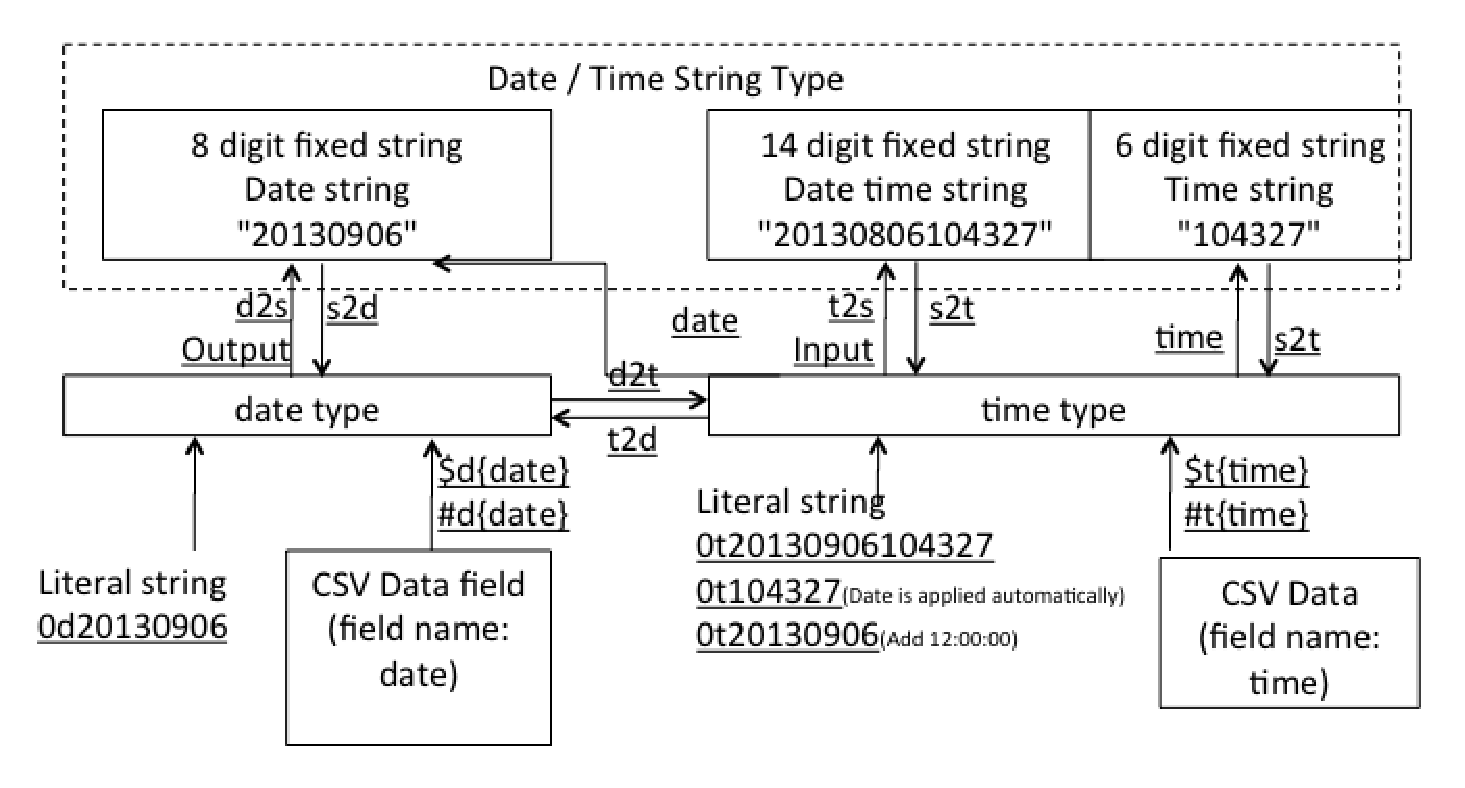
\includegraphics[scale=.50]{figure/datetime/datetime.eps}
\caption{The relationship among time type, date type and various functions using September 6, 2013 at 43 minutes, 27 seconds. The solid line box indicates actual data, the dotted line indicate the functions. \label{fig:mcal_datetime}}
\end{center}
\end{figure}

Other than using fixed length character string as a standard for date/time, user can use Julian day (e.g. continuous count of days since Julian period such as January 1, 4713 BC) or UNIX time (e.g. number of seconds that have elapsed since 00:00:00 Coordinated Universal Time (UTC), Thursday, 1 January 1970) as a signed integer to represent date and time.  The command supports Julian day and UNIX time, as well as conversion functions of date and time data type.   

The mcal command uses an internal date/time format which is based on the Gregorian calendar, thus the date range is limited from January 1,1400 to December 31,9999. Since UNIX time is a signed integer data type of 32 bits, the  furthest time that can be represented this way is 03:14:07 UTC on Tuesday, 19 January 2038, date beyond this point will be interpreted incorrectly due to integer overflow. The drawback of using UNIX time and Julian day is that one will not be able to tell the date and time by looking at the number. 

%\end{document}
